\chapter{Estados}
\section{Introducción}
A medida que se realiza una solución a un problema, los objetos deberán interactuar para llegar a esta solución, y en medio de esas interacciones, habrán acciones que incentiven el cambio de estado de uno o varios de esos objetos
\newpage
\section{Marco Teórico}

\section{Diagramas de estado}
Abarcando el problema que se esta resolviendo, se determinó que el objeto al cual se le deben aclarar sus estados, es el de tarea, pues hace parte fundamental en la solución del problema, así que el entendimiento de sus estados a lo largo de la ejecución del software que pretende implementarla será crucial.

\begin{figure}[H]
	\centering
	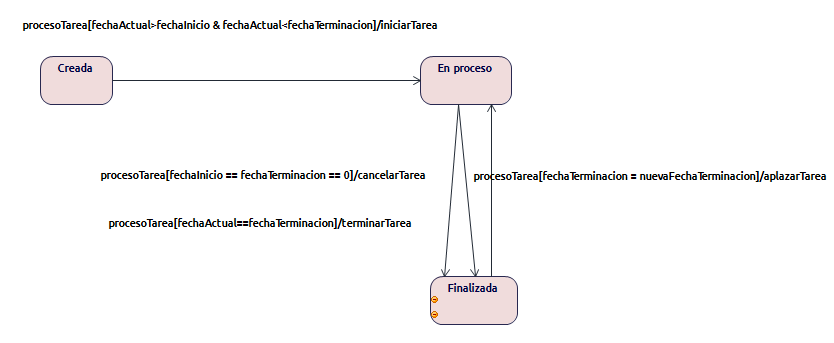
\includegraphics[width=1\linewidth]{diseno/estados/imgs/estadosTarea}
	\caption{Diagrama de estados para el objeto Tarea.}
	\label{fig:gantt}
\end{figure}

Cabe mencionar, de manera obligatoria, que este diagrama tendrá su correspondiente planeación estructural, que en otras palabras vendría a ser su espacio en el diagrama de clases de toda la solución. Para esto, existe un patrón de comportamiento, que precisamente tiene como objetivo cumplir el principio de diseño abierto/cerrado en el contexto de estados de un objeto.

\begin{figure}[H]
	\centering
	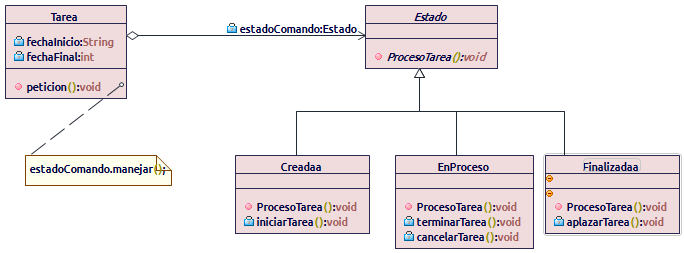
\includegraphics[width=1\linewidth]{diseno/estados/imgs/PatronState}
	\caption{Patrón state para solucionar los estados del objeto Tarea.}
	\label{fig:gantt}
\end{figure}

\begin{figure}[H]
	\centering
	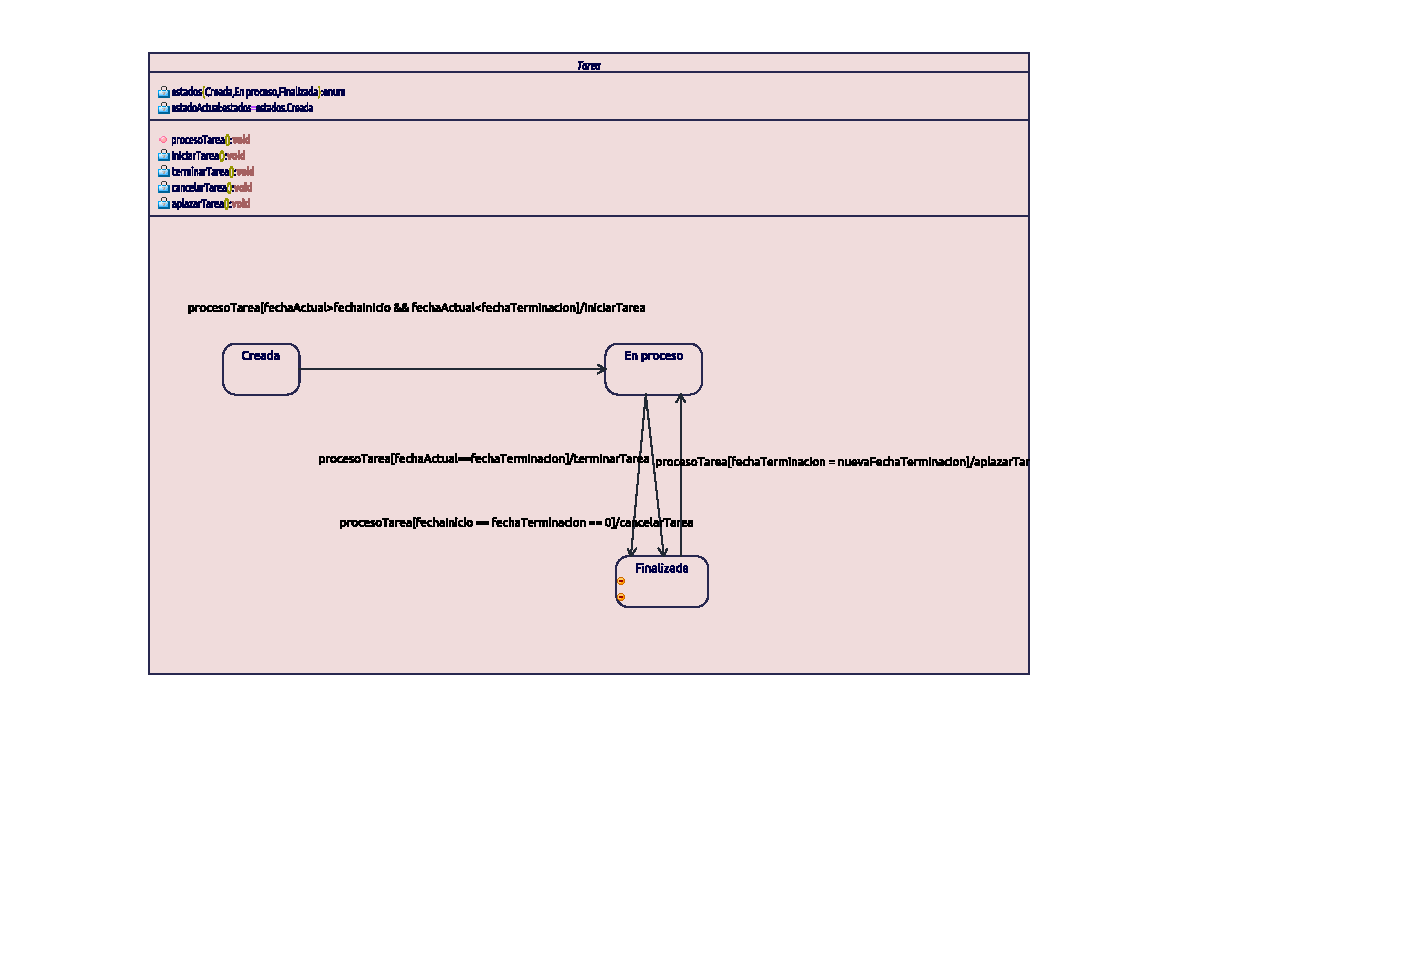
\includegraphics[width=1\linewidth]{diseno/estados/imgs/loquesea.pdf}
	\caption{Detalle de la clase Tarea bajo el contexto del patrón Estado.}
	\label{fig:gantt}
\end{figure}